\documentclass[aspectratio=169,11pt]{beamer}

\usepackage[spanish,es-nodecimaldot]{babel}
\usepackage{amsmath,amssymb,graphicx}
\usepackage{lmodern}
\usepackage{pgfplots}
\pgfplotsset{compat=1.18}

% Paleta en variaciones de azul
\definecolor{AzulNoche}{HTML}{082F49}
\definecolor{AzulProfundo}{HTML}{0C4A6E}
\definecolor{AzulMedio}{HTML}{0369A1}
\definecolor{AzulVivo}{HTML}{0284C7}
\definecolor{AzulClaro}{HTML}{38BDF8}
\definecolor{AzulHielo}{HTML}{E0F2FE}
\definecolor{Fondo}{HTML}{F8FBFF}
\definecolor{Gris}{HTML}{475569}

\setbeamercolor{normal text}{fg=AzulNoche,bg=Fondo}
\setbeamercolor{structure}{fg=AzulMedio}
\setbeamercolor{frametitle}{fg=AzulNoche,bg=Fondo}
\setbeamercolor{block title}{fg=white,bg=AzulProfundo}
\setbeamercolor{block body}{fg=AzulNoche,bg=AzulHielo}
\setbeamercolor{alerted text}{fg=AzulMedio}
\setbeamertemplate{navigation symbols}{}
\setbeamertemplate{items}[circle]
\setbeamertemplate{frametitle}{%
  \vspace{0.22cm}\insertframetitle\par\vspace{0.05cm}%
  {\color{AzulClaro}\rule{1.30cm}{1.5pt}}}
\setbeamertemplate{footline}{%
  \begin{beamercolorbox}[wd=\paperwidth,ht=2.7ex,dp=1.2ex,leftskip=.55cm,rightskip=.55cm]{author in head/foot}%
  \color{Gris}\scriptsize Acemoglu, Kong y Ozdaglar (2026) - NBER WP 34910
  \hfill\textcolor{AzulMedio}{\insertframenumber/8}
  \end{beamercolorbox}}
\setbeamerfont{title}{size=\fontsize{25}{29}\selectfont,series=\bfseries}
\setbeamerfont{frametitle}{size=\Large,series=\bfseries}
\setbeamerfont{block title}{size=\normalsize,series=\bfseries}

\newcommand{\azul}[1]{\textcolor{AzulMedio}{\textbf{#1}}}
\newcommand{\repo}{\href{https://github.com/isisroquet-mi/ai-04-acemoglu}{github.com/isisroquet-mi/ai-04-acemoglu}}

\pgfplotsset{
  grafico/.style={
    axis lines=left,
    axis line style={AzulNoche,semithick},
    tick style={AzulNoche},
    tick label style={font=\scriptsize,color=AzulNoche},
    label style={font=\scriptsize,color=AzulNoche},
    title style={font=\small\bfseries,color=AzulProfundo},
    legend style={font=\scriptsize,draw=none,fill=none},
    grid=major,
    grid style={AzulHielo},
    clip=false
  }
}

\title{IA, cognición humana y colapso del conocimiento}
\subtitle{Repositorio 4 - Modelo, resultado y lectura crítica}
\author{Isis Roque}
\date{NBER Working Paper No. 34910 - febrero de 2026}

\begin{document}

% 1. Portada
\begingroup
\setbeamercolor{background canvas}{bg=AzulNoche}
\begin{frame}[plain]
  \vfill
  \hspace{0.65cm}\begin{minipage}{0.84\paperwidth}
    {\color{AzulClaro}\rule{1.6cm}{2pt}}\\[0.45cm]
    {\usebeamerfont{title}\color{white}\inserttitle\par}
    \vspace{0.34cm}
    {\large\color{AzulHielo}\insertsubtitle\par}
    \vspace{0.85cm}
    {\normalsize\color{white}\insertauthor\par}
    {\small\color{AzulHielo}\insertdate\par}
    \vspace{0.45cm}
    {\small\color{AzulClaro}\repo}
  \end{minipage}
  \vfill
\end{frame}
\endgroup

% 2. Artículo y problema del agente
\begin{frame}{El artículo y el problema del agente}
\begin{block}{Pregunta}
¿La IA agéntica mejora las decisiones presentes a costa del aprendizaje humano que sostiene el conocimiento colectivo?
\end{block}

\begin{columns}[T,onlytextwidth]
\column{0.56\textwidth}
\azul{Elección privada}
{\small
\[
\begin{aligned}
\max_{e_{i,t}\ge 0}\ U_{i,t}
={}&f(0,0)+G(X_t)\Delta_G\\
&+G(X_t)G(Y_{i,t})\Delta_X-\frac{e_{i,t}^{\alpha}}{\alpha},
\qquad \alpha>1.
\end{aligned}
\]}
\[
Y_{i,t}=\sigma^{-2}+\lambda_I e_{i,t}+\tau_A.
\]

\column{0.40\textwidth}
\azul{Dos conocimientos}
\begin{itemize}\small
  \item $X_t$: conocimiento general heredado y compartido.
  \item $Y_{i,t}$: información específica del contexto.
  \item $e_{i,t}$ produce una señal privada y una señal pública ``delgada''.
\end{itemize}
\end{columns}

\vspace{0.05cm}
{\small\color{Gris}\textbf{Externalidad:} el agente internaliza el beneficio privado de aprender, pero no el aporte de su señal al conocimiento de cohortes futuras.}
\end{frame}

% 3. Resultado principal y condiciones
\begin{frame}{Resultado principal y condiciones}
\begin{columns}[T,onlytextwidth]
\column{0.47\textwidth}
\azul{Tensión estática: Observación 1}
\[
\frac{\partial U}{\partial e}
=\Delta_XG(X)\lambda_I g(Y)-e^{\alpha-1}.
\]
\[
\frac{\partial^2U}{\partial e\,\partial X}
=\Delta_X\lambda_I g(X)g(Y)>0,
\]
\[
\frac{\partial^2U}{\partial e\,\partial\tau_A}
=\Delta_XG(X)\lambda_I g'(Y)<0.
\]
{\small Condiciones: $\Delta_X>0$, $\lambda_I>0$, $g>0$, $g'<0$ y costo convexo $\alpha>1$. Así, $e^*$ aumenta con $X$ y disminuye con $\tau_A$.}

\column{0.49\textwidth}
\azul{Dinámica: cuándo aparece el colapso}
\begin{itemize}\small
  \item Si $\alpha-1>\tfrac14$ ($\varepsilon<4$), todo $X_1>0$ converge al único estado estable de conocimiento alto $\bar X_h>0$.
  \item Si $\alpha-1<\tfrac14$ ($\varepsilon>4$) y $\tau_A<\tau_A^c$, existen $0<\bar X_m<\bar X_h$: $X_1<\bar X_m$ converge a $0$ y $X_1>\bar X_m$ converge a $\bar X_h$.
  \item Si $\alpha-1<\tfrac14$ y $\tau_A>\tau_A^c$, $\bar X=0$ es el único estado estacionario y es globalmente estable.
\end{itemize}
\vspace{0.08cm}
{\footnotesize\color{Gris}El paper usa desigualdades estrictas. El caso frontera $\alpha-1=\tfrac14$ y la igualdad $\tau_A=\tau_A^c$ no forman parte de estas proposiciones.}
\end{columns}
\end{frame}

% 4. Lo que hice
\begin{frame}{Lo que hice}
\begin{columns}[T,onlytextwidth]
\column{0.48\textwidth}
\azul{Lectura y verificación}
\begin{itemize}\footnotesize
  \item Trabajé con el NBER Working Paper No. 34910, febrero de 2026, 69 páginas y no revisado por pares.
  \item Lo contrasté con la versión del 5 de mayo de 2026: mismo título, autores, 69 páginas y argumento central. Cambia la portada, la redacción y la parametrización $\alpha-1$ frente a $\varepsilon=1/(\alpha-1)$.
  \item Derivé la Observación 1 y separé el efecto directo e indirecto de $\tau_A$ sobre el bienestar.
\end{itemize}

\column{0.48\textwidth}
\azul{Qué demuestra y qué supone}
\begin{block}{Demostrado dentro del modelo}
\small La IA agéntica reduce el retorno marginal del esfuerzo. Bajo las condiciones de elasticidad y precisión, puede eliminar el equilibrio de conocimiento alto.
\end{block}
\begin{block}{Dependencia crítica de supuestos}
\small La Sección 5 relaja agregación, datos sintéticos y separabilidad imperfecta, pero mantiene $\Delta_I=0$ y $\Delta_X>0$. Con $\Delta_I>0$, la información específica podría conservar valor aun con poco conocimiento general.
\end{block}
\end{columns}
\end{frame}

% 5. Dónde no creí en la IA
\begin{frame}{Dónde no creí en la IA}
\begin{columns}[T,onlytextwidth]
\column{0.42\textwidth}
\azul{La intuición que puse a prueba}

{\footnotesize ``Más precisión de la IA siempre aumenta el bienestar.''}

\vspace{-0.03cm}
{\scriptsize
\[
\begin{aligned}
\frac{d\bar U^+}{d\tau_A}
={}&\underbrace{G(\bar X_h)\Delta_Xg(\bar Y_h)}_{\text{directo }>0}\\
&+\underbrace{g(\bar X_h)\big[\Delta_G+G(\bar Y_h)\Delta_X\big]
\frac{d\bar X_h}{d\tau_A}}_{\text{indirecto }<0}.
\end{aligned}
\]}
{\tiny Con el Supuesto 2, $\sigma^{-2}\ge\sqrt2-1$, $\bar U^+(\tau_A)$ tiene un pico único.}\par
\vspace{0.02cm}
{\scriptsize\color{AzulProfundo}\textbf{Veredicto: incompleta.} El efecto indirecto puede dominar.}

\column{0.54\textwidth}
\centering
\IfFileExists{hand/Derivación_Manual.pdf}{%
  \fcolorbox{AzulClaro}{white}{\includegraphics[page=3,width=0.96\linewidth,height=0.61\textheight,trim=30 425 30 28,clip,keepaspectratio]{hand/Derivación_Manual.pdf}}%
}{%
  \IfFileExists{derivacion-bienestar.png}{%
    \fcolorbox{AzulClaro}{white}{\includegraphics[width=0.96\linewidth,height=0.61\textheight,trim=80 520 80 35,clip,keepaspectratio]{derivacion-bienestar.png}}%
  }{%
    \fcolorbox{AzulClaro}{white}{\parbox[c][0.55\textheight][c]{0.92\linewidth}{\centering\color{Gris}Inserte aquí la página 3 de la derivación manual.}}%
  }%
}

{\tiny\color{Gris}Derivación manual de Isis Roque, p.~3: efecto directo $>0$ e indirecto $<0$.}
\end{columns}
\end{frame}

% 6. Dinámica y alpha
\begin{frame}{Dinámica: el papel de $\alpha$}
\vspace{-0.08cm}
{\footnotesize Los estados estacionarios aparecen donde $F(X)$ corta la línea de 45 grados. Se fija $\tau_A=0.48$ y se modifica únicamente $\alpha$. El panel derecho amplía la región de los tres cruces.}

\begin{columns}[T,onlytextwidth]
\column{0.49\textwidth}
\centering
\begin{tikzpicture}
\begin{axis}[
  grafico,width=\linewidth,height=0.50\textheight,
  xmin=0,xmax=0.62,ymin=0,ymax=0.62,
  xtick={0,0.2,0.4,0.6},ytick={0,0.2,0.4,0.6},
  xlabel={$X_t$},ylabel={$X_{t+1}$},
  title={$\alpha=1.50$: único cruce positivo}
]
\addplot[AzulClaro,densely dashed,semithick] coordinates {(0,0) (0.62,0.62)};
\addplot[AzulProfundo,very thick,smooth] coordinates {
(0.000,0.00000) (0.025,0.08249) (0.050,0.14655) (0.075,0.19830)
(0.100,0.24133) (0.125,0.27789) (0.150,0.30949) (0.175,0.33720)
(0.200,0.36178) (0.225,0.38378) (0.250,0.40365) (0.275,0.42171)
(0.300,0.43824) (0.325,0.45344) (0.350,0.46749) (0.375,0.48054)
(0.400,0.49269) (0.425,0.50406) (0.450,0.51472) (0.475,0.52475)
(0.500,0.53421) (0.525,0.54315) (0.550,0.55163) (0.575,0.55967)
(0.600,0.56733)};
\addplot[only marks,mark=*,mark size=2.2pt,AzulProfundo] coordinates {(0.5524,0.5524)};
\node[font=\scriptsize,anchor=west,text=AzulProfundo] at (axis cs:0.558,0.5524) {$\bar X_h$};
\end{axis}
\end{tikzpicture}

\column{0.49\textwidth}
\centering
\begin{tikzpicture}
\begin{axis}[
  grafico,width=\linewidth,height=0.50\textheight,
  xmin=0,xmax=0.36,ymin=0,ymax=0.36,
  xtick={0,0.1,0.2,0.3},ytick={0,0.1,0.2,0.3},
  xlabel={$X_t$},ylabel={$X_{t+1}$},
  title={$\alpha=1.20$: tres cruces}
]
\addplot[AzulClaro,densely dashed,semithick] coordinates {(0,0) (0.36,0.36)};
\addplot[AzulVivo,very thick,smooth] coordinates {
(0.000,0.00000) (0.015,0.01490) (0.030,0.02979) (0.045,0.04480)
(0.060,0.06000) (0.075,0.07542) (0.090,0.09103) (0.105,0.10679)
(0.120,0.12267) (0.135,0.13859) (0.150,0.15449) (0.165,0.17029)
(0.180,0.18594) (0.195,0.20138) (0.210,0.21656) (0.225,0.23143)
(0.240,0.24596) (0.255,0.26013) (0.270,0.27391) (0.285,0.28729)
(0.300,0.30027) (0.315,0.31283) (0.330,0.32500) (0.345,0.33676)
(0.360,0.34813)};
\draw[densely dotted,Gris] (axis cs:0.0599,0) -- (axis cs:0.0599,0.0599);
\draw[densely dotted,Gris] (axis cs:0.3018,0) -- (axis cs:0.3018,0.3018);
\addplot[only marks,mark=*,mark size=2.2pt,AzulProfundo] coordinates {(0,0) (0.3018,0.3018)};
\addplot[only marks,mark=o,mark size=2.5pt,very thick,AzulClaro] coordinates {(0.0599,0.0599)};
\node[font=\tiny,anchor=south west,text=AzulMedio] at (axis cs:0.064,0.0599) {$\bar X_m\!\approx\!0.060$};
\node[font=\tiny,anchor=north east,text=AzulProfundo] at (axis cs:0.297,0.3018) {$\bar X_h\!\approx\!0.302$};
\end{axis}
\end{tikzpicture}
\end{columns}

\vspace{-0.08cm}
{\footnotesize Con $\alpha=1.20$, los cruces son $\bar X_\ell=0$, $\bar X_m\approx0.060$ y $\bar X_h\approx0.302$. El punto intermedio separa las dos cuencas de atracción.}

{\tiny\color{Gris}Simulación ilustrativa: $\Delta_X=6$, $\lambda_I=I=\Sigma^2=1$, $\lambda_G=2$ y $\sigma^{-2}=0.5$.}
\end{frame}

% 7. Umbral de colapso
\begin{frame}{Umbral de colapso}
\begin{columns}[T,onlytextwidth]
\column{0.66\textwidth}
\centering
\begin{tikzpicture}
\begin{axis}[
  grafico,width=\linewidth,height=0.58\textheight,
  xmin=0,xmax=0.55,ymin=0,ymax=0.55,
  xtick={0,0.1,0.2,0.3,0.4,0.5},ytick={0,0.1,0.2,0.3,0.4,0.5},
  xlabel={$X_t$},ylabel={$X_{t+1}$},
  legend style={font=\tiny,at={(0.02,0.98)},anchor=north west,row sep=-1pt}
]
\addplot[Gris,densely dashed,semithick] coordinates {(0,0) (0.55,0.55)};
\addlegendentry{Línea de 45 grados}
\addplot[AzulProfundo,very thick,smooth] coordinates {
(0.000,0.00000) (0.025,0.02503) (0.050,0.05096) (0.075,0.07820)
(0.100,0.10657) (0.125,0.13565) (0.150,0.16486) (0.175,0.19368)
(0.200,0.22167) (0.225,0.24853) (0.250,0.27406) (0.275,0.29818)
(0.300,0.32086) (0.325,0.34215) (0.350,0.36208) (0.375,0.38075)
(0.400,0.39823) (0.425,0.41462) (0.450,0.42999) (0.475,0.44443)
(0.500,0.45802) (0.525,0.47081) (0.550,0.48288)};
\addlegendentry{$\tau_A=0.40<\tau_A^c$}
\addplot[AzulVivo,very thick,densely dotted,smooth] coordinates {
(0.000,0.00000) (0.025,0.02473) (0.050,0.04938) (0.075,0.07427)
(0.100,0.09941) (0.125,0.12469) (0.150,0.14995) (0.175,0.17497)
(0.200,0.19951) (0.225,0.22342) (0.250,0.24652) (0.275,0.26874)
(0.300,0.29001) (0.325,0.31027) (0.350,0.32955) (0.375,0.34784)
(0.400,0.36519) (0.425,0.38163) (0.450,0.39720) (0.475,0.41195)
(0.500,0.42593) (0.525,0.43919) (0.550,0.45177)};
\addlegendentry{$\tau_A=\tau_A^c\approx0.526$}
\addplot[AzulClaro,very thick,densely dashed,smooth] coordinates {
(0.000,0.00000) (0.025,0.02458) (0.050,0.04860) (0.075,0.07228)
(0.100,0.09568) (0.125,0.11882) (0.150,0.14165) (0.175,0.16411)
(0.200,0.18613) (0.225,0.20762) (0.250,0.22853) (0.275,0.24879)
(0.300,0.26836) (0.325,0.28722) (0.350,0.30534) (0.375,0.32272)
(0.400,0.33937) (0.425,0.35530) (0.450,0.37053) (0.475,0.38508)
(0.500,0.39898) (0.525,0.41226) (0.550,0.42495)};
\addlegendentry{$\tau_A=0.65>\tau_A^c$}
\addplot[only marks,mark=o,mark size=2.3pt,very thick,AzulClaro] coordinates {(0.0224,0.0224)};
\addplot[only marks,mark=*,mark size=2.1pt,AzulProfundo] coordinates {(0.3945,0.3945)};
\addplot[only marks,mark=*,mark size=2.1pt,AzulVivo] coordinates {(0.1634,0.1634)};
\end{axis}
\end{tikzpicture}

\column{0.30\textwidth}
{\small\azul{Cambio en $F(X)$}}

{\scriptsize Se mantiene $\alpha=1.20$. Un aumento de $\tau_A$ reduce el esfuerzo humano y desplaza $F(X)$ hacia abajo.}

\vspace{0.05cm}
{\small
\[
\tau_A^c\approx0.526,
\qquad \bar X^c\approx0.163.
\]}

{\scriptsize
\textbf{$\tau_A<\tau_A^c$:} dos equilibrios positivos.\\[0.08cm]
\textbf{$\tau_A=\tau_A^c$:} los dos se unen por tangencia.\\[0.08cm]
\textbf{$\tau_A>\tau_A^c$:} solo permanece $\bar X=0$.
}
\end{columns}
\end{frame}

% 8. Path dependence
\begin{frame}{Dependencia de la condición inicial}
\begin{columns}[T,onlytextwidth]
\column{0.70\textwidth}
\centering
\begin{tikzpicture}
\begin{axis}[
  grafico,width=\linewidth,height=0.60\textheight,
  xmin=0,xmax=400,ymin=0,ymax=0.34,
  xtick={0,100,200,300,400},ytick={0,0.1,0.2,0.3},
  xlabel={Cohorte, $t$},ylabel={Conocimiento general, $X_t$},
  legend style={font=\scriptsize,at={(0.02,0.98)},anchor=north west,row sep=1pt,fill=white,fill opacity=0.88,text opacity=1}
]
\addplot[AzulClaro,densely dashed,semithick] coordinates {(0,0.0599) (400,0.0599)};
\addlegendentry{Umbral $\bar X_m\approx0.060$}
\addplot[AzulProfundo,very thick,smooth] coordinates {
(0,0.04000) (20,0.03544) (40,0.03094) (60,0.02676) (80,0.02306)
(100,0.01989) (120,0.01723) (140,0.01502) (160,0.01319)
(180,0.01167) (200,0.01040) (220,0.00934) (240,0.00844)
(260,0.00767) (280,0.00702) (300,0.00645) (320,0.00596)
(340,0.00553) (360,0.00515) (380,0.00482) (400,0.00452)};
\addlegendentry{$X_1=0.04<\bar X_m$}
\addplot[AzulVivo,very thick,smooth] coordinates {
(0,0.08000) (20,0.09833) (40,0.14956) (60,0.26464) (80,0.29994)
(100,0.30170) (120,0.30177) (140,0.30177) (160,0.30177)
(180,0.30177) (200,0.30177) (220,0.30177) (240,0.30177)
(260,0.30177) (280,0.30177) (300,0.30177) (320,0.30177)
(340,0.30177) (360,0.30177) (380,0.30177) (400,0.30177)};
\addlegendentry{$X_1=0.08>\bar X_m$}
\addplot[AzulMedio,densely dotted,semithick] coordinates {(0,0.3018) (400,0.3018)};
\end{axis}
\end{tikzpicture}

\column{0.26\textwidth}
{\footnotesize Con $\alpha=1.20$ y $\tau_A=0.48$ existen tres estados estacionarios:}
{\small
\[
\begin{aligned}
\bar X_m&\approx0.0599,\\
\bar X_h&\approx0.3018.
\end{aligned}
\]}
\begin{itemize}\scriptsize
  \item $X_1=0.04$ cae gradualmente hacia $0$.
  \item $X_1=0.08$ converge hacia $\bar X_h$.
\end{itemize}

{\tiny\color{Gris}El umbral separa dos cuencas de atracción. Una diferencia inicial de $0.04$ cambia el resultado de largo plazo.}
\end{columns}
\end{frame}

\end{document}
